\documentclass[twoside,11pt,ShortChapTitles]{BYUTextbook}

\usepackage{soul}
\renewcommand{\vec}[1]{\ensuremath{\mathbf{#1}}}
\usepackage{siunitx}
\sisetup{round-mode = figures,
  round-precision = 3, scientific-notation=true}
  \usepackage{marginfix}

\usepackage{mathtools}






\setcounter{chapter}{3}

\begin{document}


\chapter[Experimental Design I]{Experimental Design I: Harmonic Oscillators (masses and springs)\label{Experimental Design}}
\section{Getting better accuracy by fitting data}
In the last lab, we used the mean and standard deviation to find a measurement and its error.  We then used our measurements and error propagation to calculate $g$ and the error in our calculation.

What if you wanted better accuracy?  One option would be to just repeat the same measurement many different times in hopes of getting a better mean value.  However, if the person doing the timing always ends the timer a little too soon, or your scale actually reads 5 kg when it should read zero, repeating the measurement won't help you gain any more accuracy.

But if you change how your measuring a little bit each time, by dropping the ball from a different height, or changing the length of your pendulum string, you can get a better calculated value, even if your measurement technique is off.  (As long as it is consistently wrong.  If your scale is 5 grams off when you weight something that is 20 grams, and 50 grams off when you weight something at 100 g, you need a new scale.)

This section will show you how.

\subsection{Linear Least Squares}

Linear least squares is the most common type of data fitting (other than just averaging) because it is fast, easy (once you get the hang of it), and it has a known solution. (It's a plug and chug formula)
Many types of fits just have a computer try a bunch of values and see which one fits the best.  Sometimes the computer will miss the actual best fit for something that is just better than the choices around it, and even if the computer does find the best fit, it will take much longer to get there.

Here is the basics of how least squares fitting works.  Imagine that you've taken the data shown below:

\begin{center}
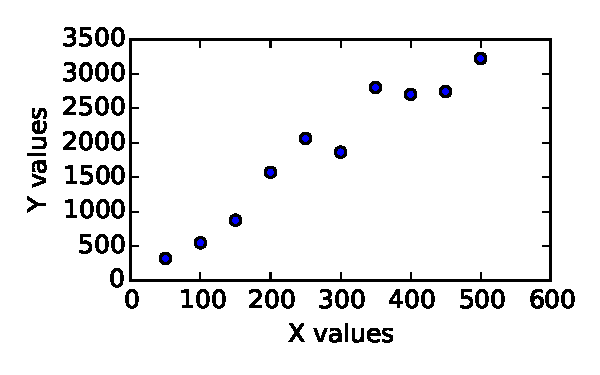
\includegraphics{Lab4_figs/dataScatter.pdf}
\end{center}

The data wiggles all over the place, but it is easy to see that it generally follows a line.  Therefore, we'd predict that our data should match:
\[y=mx+b\]
But there is no single line that will go through every single data point.  There's always a little bit of error, often written as $\chi$, and it represents the little green lines in the figure below:
\begin{center}
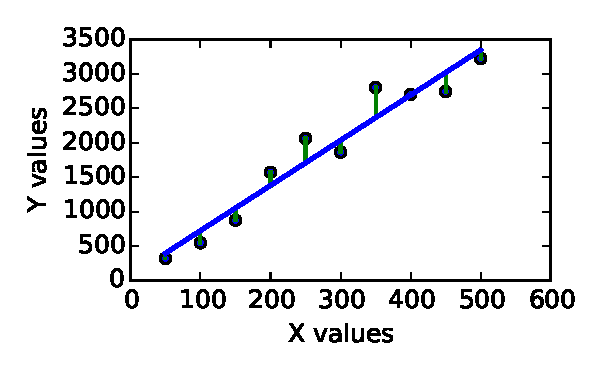
\includegraphics{Lab4_figs/dataWfit.pdf}
\end{center}

My data actually matches this equation:
\[y_i=mx_i+b+\chi_i\]
Where $y_i$ is the $y$ value corresponding to each individual $x$ value, $x_i$.  $\chi_i$ gives how far away each data point is from the line. We can solve for how far away from the line each data point is:
\[\chi_i=y_i-b-mx_i\]
and come up with a function that gives us a total error:
\[E_{tot}=\sum_i^N \chi_i^2 = \sum_i^N (y_i-b-mx_i)^2\]
which is just the sum of how far off every single data point is from the line.  We use $\chi_i^2$ as an easy way to get the absolute value of each error.  We really only care about how far each data point is from the line, not whether it is above or below the line.  Using calculus, we can find the slope and intercept of the line that will minimize the our total error.  To minimize, we just take the derivative of our error function with respect to the thing we want to minimize, and set it equal to zero:
\[\frac{\partial E_{tot}}{\partial m}=0;\,\,\,\frac{\partial E_{tot}}{\partial b}=0\]
If you do those derivatives, and use the two equations to solve for $m$ and $b$, you get this:
\[m=\frac{\left<xy\right>-\left<x\right>\left<y\right>}{\left<x^2\right>-\left<x\right>^2}\]
\[b=\left<y\right>-m\left<x\right>\]
where $m$ and $b$ are the slope and intercept of the line that gets closest to all of the data points.  The $\left<\right>$ symbols mean the average of the thing inside. $\left<x\right>$ is the average of all the $x$s.  To calculate $\left<xy\right>$ you'd multiply each $x$ value by its corresponding $y$ value, then take the average.
Using error propagation, you can find the errors in you fit.  The error in the slope is:
\[\sigma_m=\frac{\sigma_y}{\sqrt{N\left(\left<x^2\right>-\left<x\right>^2\right)}}\]
and the error in the intercept is:
\[\sigma_b=\sigma_y\sqrt{\frac{\left<x^2\right>}{N\left(\left<x^2\right>-\left<x\right>^2\right)}}\]
$\sigma_y$ represents the average error of each y value, and is calculated using:
\[\sigma_y=\sqrt{\frac{1}{N-2}\sum_i^N \left(y_i-b-mx_i\right)^2}\]

For reference, here is a figure with the best fit line for to the data.  The red lines mark the high/low values given by the error in the slope:
\begin{center}
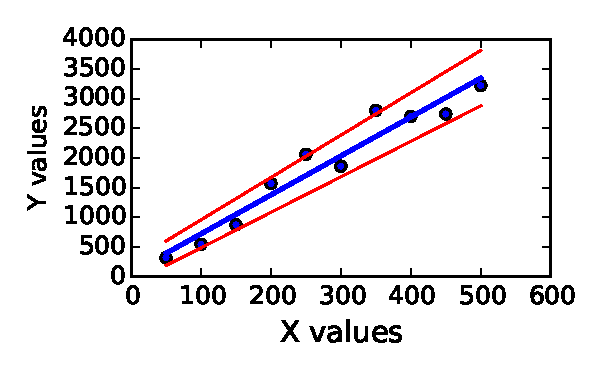
\includegraphics{Lab4_figs/dataWfitRange.pdf}
\end{center}

Here's an example of a Python function that takes in x and y values and returns the slope and intercept of the best fit line, with their errors.  It would be very go practice to read through it and see if you can figure out what each line does.
\begin{Verbatim}
def linearLeastSquares(x,y):
    #Import numpy
    import numpy as np
    #Get the number of data points
    N=len(x)

    #Make sure x and y are numpy arrays to make array math easy
    x=np.asarray(x)
    y=np.asarray(y)

    #Calculate the average values needed to find the slope and intercept
    xbar=np.mean(x) #Average Value of the xdata
    ybar=np.mean(y) #Average value of the y data
    xbar2=np.mean(x**2) #Average value of the xdata squared
    xybar=np.mean(x*y) #Average value of xdata*ydata



    #Use the linear least squares formula to calculate
    #the slope and the intercept of the best fit line
    slope=(xybar-xbar*ybar)/(xbar2-xbar**2)
    intercept=ybar-slope*xbar

    #This section estimates the error in the fit =========================

    #Calculate the variance in the fit
    #Calculate the stuff inside the sum first to make the code easier to read
    sigmaYinsideSum = np.square(y-intercept-slope*x)

    #Get the uncertaintiy in the measurements (variance)
    sigmaY=np.sqrt(np.sum(sigmaYinsideSum)/(N-2))

    #Now calculate the error in the slope and intercept
    sigmaSlope = sigmaY/np.sqrt(N*(xbar2-xbar**2))
    sigmaIntercept = sigmaY*np.sqrt(xbar2/(N*(xbar2-xbar**2)))

    #End of error estimating section =====================================

    #Now return the slope and intercept, with their error as a list of lists

    return [
           [slope,sigmaSlope],
           [intercept,sigmaIntercept]
           ]
\end{Verbatim}





\subsection{Linearizing equations}
One of the major downsides to linear least squares fitting is that it only works on lines.  While most of the relationships in physics aren't readily linear, we can tweak them to make them linear.  We call this ``linearizing the equation".

Here's an example.  We take a video of a ball, dropped from rest, and measure how far it has fallen in each frame.  In this instance, we'd predict that the relationship between the distance fallen, $y$ and the time $t$ would be:
\[y=\frac{1}{2}gt^2\]
where $g$ is the acceleration due to gravity.  The plot of $y$ vs $t$ is looks like this:
\begin{center}
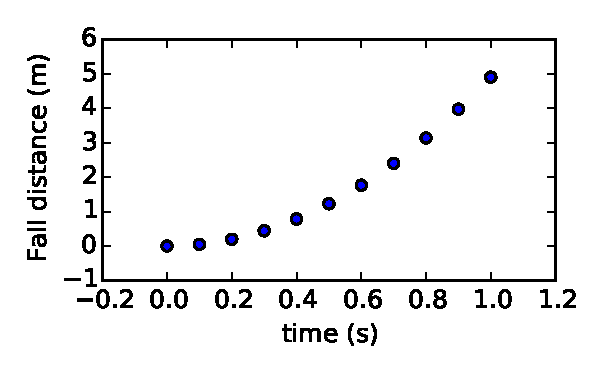
\includegraphics{Lab4_figs/yvst.pdf}
\end{center}
That is definitely not linear, but we can tweak it so that it is.  Here are the steps:
\begin{enumerate}
\item First isolate the dependent variable, or the thing you measured.  In this case, that would be our distance fallen, $y$.
\item See if it looks like a line.  Here's how you can tell. In $y=mx+b$ we have three parts that determine $y$: $m$ and $b$ are constant, $x$ is something that changes.  In our example, we change $t$ as we advance frame by frame, that's called our independent variable.
\end{enumerate}
So, let's check our equation. Do we have a constant that multiplies some function of our independent variable.  In this case, we have $\frac{1}{2}a$ as a constant, and $t^2$ is a function of our independent variable; therefore, we make our slope $m=\frac{1}{2}a$ and our x values $x=t^2$. Since we don't have anything that we are adding, $b=0$.  To add an extra check to our work, here is a plot of $y$ vs $t^2$:
\begin{center}
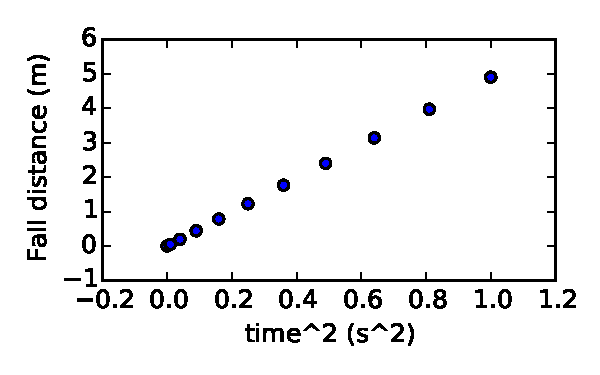
\includegraphics{Lab4_figs/yvst2.pdf}
\end{center}
which is very much linear.

As another example, suppose we wanted to find the density of copper.  To that end, we melted some copper and let it drip out a small hole, and let the drops fall as they cooled.  A drop will form an almost perfect sphere. (This is actually how they make ball bearings.)  By changing the size of the whole, you change how much mass the droplet can accumulate before it falls.  (Making mass our independent variable.)  As we vary the size of the hole, we record the mass and radius of the copper ball bearings.  Density, $\rho$, obeys the following relationship:
\[\rho = \frac{m}{V}=\frac{m}{(4/3)\pi r^3}\]

If we solve for our dependent variable, $r$, we get:
\[r^3=\frac{m}{(4/3)\pi\rho}\]
Notice that I left $r^3$, rather than solving completely for $r$.  You only need to isolate your dependent variable, not solve for it.  Our only thing that is changing on the right hand side of our equation is $m$, so our $y$ axis should be $r^3$, our $x$ axis will be $m$, and our slope will be $1/\left[\left(4/3\right)\pi\rho\right]$.

Now, we could solve completely for $r$ and get a valid result.  If we use:
\[r=\left[\frac{m}{(4/3)\pi\rho}\right]^{1/3}\]
then $r$ would be our $y$ values, $m^{1/3}$ would be our $x$ values, and $\left[\left(4/3\right)\pi\rho\right]^{-1/3}$ would be our slope.


\section{Introduction to Lab}

We are going to tackle the subject of experimental design today, but it helps
to have an experiment in mind. You are learning or have learned Hook's law for
springs in your PH121 class. You understand that when we attach a mass to a
spring and stretch or compress a spring we have a force
\[
F_{s}=-kx
\]
on the mass, where by $k$ we mean the spring stiffness constant, and by $x$ we
mean the displacement from the equilibrium position of the mass-spring system.
We can make such a system oscillate. This is really a PH123 problem, but let's
pretend that we are scientists in Newton's day and we don't know much about
oscillation (because most of us don't yet). We wish to find out more. We know
that if we build a mass-spring system we can get oscillation and we define the
time it takes for the mass to travel through one full oscillation (so the
mass, say, starts from the highest point and it returns to it's highest point)
as the \emph{period} of oscillation and abbreviate it with the letter $T.$
\begin{center}
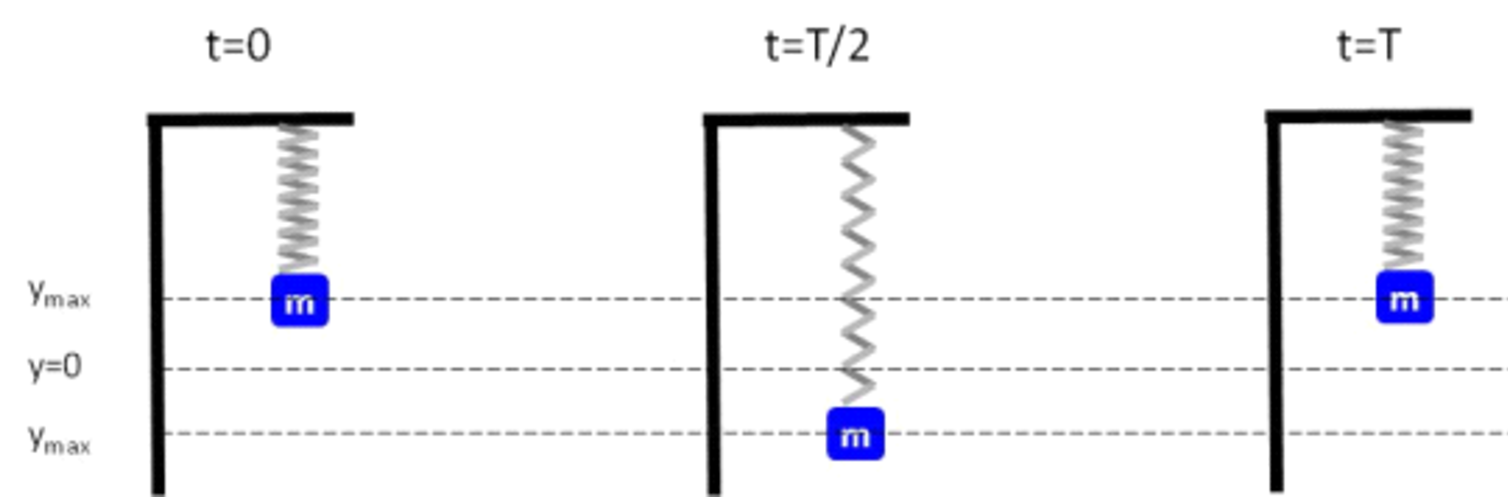
\includegraphics[
natheight=1.248800in,
natwidth=3.767100in,
height=1.2842in,
width=3.8156in
]
{Lab4_figs/massOnSpring.png}
\end{center}
Let's further pretend that you have read Hook's work and from this work have
reason to believe that period might be proportional to the square root of the
mass.
\[
T\propto\sqrt{m}
\]
You want to verify this report and build your own model for the period of
oscillation of a mass-spring system. You will use this model to make
predictions, and by doing so, you will see how well your model works. This is
what we want to investigate, now let's see how to design our experiment.

\section{Designing an experiment}

One of our objectives in this course is to learn how to design an experiment
so that it will be successful.

Back in grade-school, an experiment was any science related activity (the
proverbial building of a volcano model was considered an experiment). But for
a scientist, an experiment is a specific thing. It is the testing of a
hypothesis. You must test a hypothesis with care because the entire foundation
of science depends on the integrity of how we do this testing.

In today's lab I will give you a hypothesis to test (the period of oscillation
for a mass-spring system depends directly on the square root of the mass). The
following steps will help your experiment be successful.

\begin{enumerate}
\item Identify the system to be examined. In our case it is a mass-spring
system. We should identify all the \emph{inputs} to the system. For example,
we know there is a mass, $m$, and you have heard about a spring constant, $k.
$ There is also the force due to gravity and tension on a spring. These are
inputs. You should describe your system in your lab notebook and list the
inputs. These inputs are the things you can possibly change in the design of
your experiment.

\item Identify the model to be tested. The word \textquotedblleft
model\textquotedblright\ means our mental picture of how something works. As
physicists, we would prefer to express a model in a mathematical equation. For
example, we have a model of how force depends on acceleration. The bigger the
acceleration, the more the force. But our model also includes mass. The larger
the mass, the larger the force needed to create the same acceleration. This
mental model can be expressed in an equation
\[
F=ma
\]
It is valuable to use both the word description of the model as well as our
mathematical representation. In our case today, our mental model is that
period of oscillation for a mass-spring system depends directly on the square
root of the mass. Think about what this means. If I increase the mass, the
period should get longer. But if I\ double the mass, the period won't double.
This is a mental model that allows us to do predictions of behavior. In
physics it is almost required to reduce this model to an algebraic equation
that can be used to calculate a prediction and an uncertainty on that
prediction. For today's experiment that equation is
\[
T=C\sqrt{m}
\]
where $C$ is a factor that does not depend on mass, but for your experiment
that your group designs later in this course you will have to come up with
your own mathematical expression of your model. Record your model and the
model equation in your lab notebook.

\item Plan how you will know if you are successful in your experiment. You are
testing a hypothesis, and you are much more likely to succeed in your test if
you plan what that success would look like. One way to do this is to plan how
you will communicate your results. It is a great idea to think of what graph
you will make at the end of the experiment to communicate whether your model
works (or not). In today's experiment, a graph of $T$ vs. $m$ or even $T$
vs.$\sqrt{m}$ might be useful along with a curve fit. Notice I\ am suggesting
you plan this before you perform the experiment. I am not suggesting you
decide on what the results will be, only how you will report them. This
focuses your attention on deciding what measurement you will make. In our case
today it is hard to plot $T$ vs. $m$ if you don't measure $T$ and $m,$
planning the graph in advance helps you plan the experiment. Mock up your
graph or figure in your lab notebook. Give axis titles and even units (but of
course no data yet).

\item Rectify your equation. It would be good to be able to use a curve fit to
analyze our data. The strongest and most reliable curve fits are straight line
fits where the fit equation is something like
\[
y=mx+b
\]
So if at all possible, we would like to reduce our equation to the equation of
a straight line. In today's lab we can do this. We call this \emph{linearizing
the equation}. If we can't find a way to linearize the equation, we at least
need to render our equation into a form that we can use to predict the outcome
of our experiment. Record your new equation in your lab notebook.

\item Choose ranges of the variables. For today's experiment we might have
several, but $m$ and $k$ are principal variables. It should be clear when you
see the spring that putting a thousand kilograms of mass on the spring would
be a bad idea. but how much mass is right? What will give you good results in
testing your theory? Hooks law is not valid for all $m$ and $k$ (if you doubt
this, think of your Christmas slinky after your brother got to it; it never
looked the same again!). What values of $m$ are best for performing the
experiment? An error analysis based on your equation is invaluable in making
this decision. Changes in mass that produce a change in $T$ that is smaller
than the uncertainty in $T$ will not be noticeable. So taking measurements for
such small mass changes would be a waste of time and effort. We would like to
avoid this. Changes that are likely to break the equipment are also not
desirable. And of course you want to plan this before you do the experiment
and find that you did not get good data, and therefore must repeat all your
work! Record your variable ranges in your lab notebook. As you perform the
experiment note any deviations from this plan.

\item Plan the experimental procedure. As a group talk your way through the
experiment. You might find yourselves saying something like \textquotedblleft
then you take the stopwatch and measure the period..\textquotedblright\ and
you realize that you did not get a stop watch. For your experiment that you
design, you need to find out in advance if we have the equipment you need. So
get in the habit of working through the procedure in advance to see if you
have forgotten anything. Record your planned procedure in your lab notebook.
As you perform the experiment, note any deviations from the plan and the
reason for the deviation. Deviations are fine, just make sure you record them.

\item Perform the experiment and report on it in your lab notebook. This
involves all the things we have been including in our lab notebooks to date
\end{enumerate}

\begin{itemize}
\item Describing the goal for the work. (This is probably already done in your plan)

\item Give predictive equations and uncertainties for the predictions based on
the physical law. (This is probably already done in your plan)

\item Give your procedure you actually followed, recording what you really did
as you do it. This will probably not be just a restatement of the plan because
things will change as you go. Record the equipment used and settings, values,
etc. for that equipment. Did you learn how to use any new equipment? What did
you learn that you want to recall later (say, when taking the final, or when
you are a professional and need to use a similar piece of equipment five years
from now).

\item Record the data you used. . If you have a large set of values, you can
place them in a file, and then record the file name and location in your lab
notebook. Make sure this is a file location that does not change (emailing the
data to yourself is still not a good plan).

\item Give a record of the analysis you performed. You planned this above, now
record what you actually did

\item Give a brief statement of your results and their associated uncertainties.

\item Draw conclusions: Do your results support the theory? Why or why not?
What else did you learn along the way that you want to record. (This is where
we may compare the percent error to our relative uncertainty).
\end{itemize}

\section{Assignment}

This week's assignment follows the experimental design process outlined above.
I have mostly designed this experiment for you. So this week I want you to
identify the design parts and put them in our design process order. For our
next design lab, you will have to design the experiment yourself. This week's
lab is to get familiar with the process. Perform this experiment as a group.

\subsection{First Part: Data Collection}

\begin{enumerate}
\item Our system will be the mass-spring system and it's hanger. Obtain a set
of weights, a spring, a weight hanger, a stand, and a stopwatch. Attach the
spring to the stand, and the weight hanger to the spring. Determine the inputs
to this mass-spring system that may affect the output quantity of interest
(the period of oscillation). Determine whether each of these inputs will
affect the period of oscillation. If so, explain how you will control for that
input. If not, give justification for why you can ignore that input.

\item Build a mathematical model beginning with the suggestion you got from
reading Hook's work (above).

\item Determine how you will measure the period of oscillation. Remember that
you want to minimize the amount of uncertainty in your measurement. Techniques
we have learned in previous labs may help. Record your method. You should plan
any graphs you will make and in general plan how you will report your data and
whether or not your experiment is successful.

\item Discuss how you might go about making your equation look linear by a
proper substitution of variables. Explain why this might be useful.

\item Select a range of variables. (e.g. $m=$ $20
\operatorname{g}
$, $30
\operatorname{g}
$, $40
\operatorname{g}
$, $50
\operatorname{g}
$, and $100
\operatorname{g}
$). Don't use $80
\operatorname{g}
$ because I want to reserve this value for a special purpose below. Stop at
about $100
\operatorname{g}
.$

\item Plan your procedure and record your plan in your lab notebook.

\item Perform the experiment. Your plan probably includes determining the
period of oscillation for masses that you have selected. Be sure to record any
measurement uncertainty. Make the graphs of your data that you planned
including the appropriate error bars and a best fit line (See second part). Attach the graphs in your lab notebook.
Record what you do and highlight any deviations from your planned procedure.
Record your data or your data file name and location. Show your analysis and
give your results. Draw conclusions. We will check these conclusions in the
third part. But state whether you believe that $T\propto\sqrt{m}$
\end{enumerate}

\subsection{Second Part: fitting a line}
In order to fit a line to your data, you'll need to teach Python how to do a linear least squares fit using the equations and the example function in the lab introduction.  You will be doing many linear least squares fits, so it is in your best interest to create a least squares function in its own file that you can use in the future.  That way you don't have to copy and paste it over and over again. These steps will teach you how.
\begin{enumerate}
\item Linearize your equation.  Remember, linear least squares fitting only works on lines.
\item Type out the example program given in this lab's intro, and save it in the folder where you have been saving your other programs from lab.  Make sure that you match the indentation from the example.  Python uses indentation to tell where functions end.  Here's a quick example:
\begin{Verbatim}
def line(x,m,b):
    return m*x+b
\end{Verbatim}

Notice the difference in indentation between the two lines. The "def" command tells Python that you want to create your own function.  In this case, the function is called \code{line} and takes inputs \code{x},\code{m}, and \code{b}.  The return command tells Python what you want to get out of your function.  You could define a function this way and get the same result:

\begin{Verbatim}
def line(x,m,b):
    y=m*x+b
    return y
\end{Verbatim}

But you will get an error if you enter this:
\begin{Verbatim}
def line(x,m,b):
    y=m*x+b
return y
\end{Verbatim}
Indentation is very important in Python.  When you define a function, everything that is indented below it is counted as part of that function.  Not indenting the return statement tells Python that you've ended your function, and it won't know what to return.
Here's one more example:
\begin{Verbatim}
def line(x,m,b):
    y=m*x+b
    return y

y=line(5,2,1)
\end{Verbatim}
The previous piece of code tells Python what we want our function to be.  Then,  the very last line (notice that it is not indented) tells Python that we want to use our function, and that we want \code{x=5}, \code{m=2}, and \code{b=1}.  Python will perform the operation and save the number 11 (5*2+1) into the variable \code{y}.  Python will also treat any variables inside of functions as separate from the ones outside, meaning the \code{y} in our function is independent of the \code{y} in the last line. Once you define a function, you can use it over and over again in your program.

\item Test your function.  Put these lines of code {\em after} your function: (you only have to choose one function call, but make sure your print statements match.)
\begin{Verbatim}
xdata=[1,2,3,4,5,6]
ydata=[1,2,3,4,5,6]
#There are three different ways to call your function, pick one.
#What gets loaded where is described after the function call

fit_params = linearLeastSquares(xdata,ydata)
#With this call:
#slope will be in fit_params[0][0], the slope's error in fit_params[0][1]
#intercept will be in fit_params[1][0], the intercept's error in fit_params[1][0]

slope, intercept = linearLeastSquares(xdata,ydata)
#With this call:
#slope will be in slope[0], the slope's error in slope[1]
#intercept will be in intercept[0], the intercept's error in intercept[1]

[slope,slopeErr], [intercept,interceptErr] = linearLeastSquares(xdata,ydata)
#With this call:
#slope will be in slope, the slope's error in slopeErr
#intercept will be in intercept, the intercept's error in interceptErr

#These print statements were built using the variable names from the third function call
print('Slope: {}+/-{}'.format(slope,slopeErr))
print('Intercept: {}+/{}'.format(intercept,interceptErr))
\end{Verbatim}
If your program is working properly, it will print:
\begin{Verbatim}
Slope: 1.0+/-0.0
Intercept: 0.0+/0.0
\end{Verbatim}

\item If you are confident that your equipment is properly zeroed, you can get a more accurate fit by forcing your intercept to be zero.  Inside the same file that you typed up your \code{linearLeastSquares} function, create a second function called \code{linearLeastSquaresNoIntercept} that will do a least squares fit to a line without an intercept and return the slope and its error.

The equations for fitting a no intercept least squares line are:
\[m=\frac{\left<xy\right>}{\left<x^2\right>}\]
\[\sigma_m=\frac{\sigma_y}{\sqrt{\left<x^2\right>}}\]
\[\sigma_y=\sqrt{\frac{1}{N-1}\sum_i^N \left(y_i-mx_i\right)^2}\]

You should get a slope of 1 and an intercept of 0 if your function is working correctly.
\end{enumerate}

Now start building a script to fit this week's data.
\begin{enumerate}
\item Open up a new Python script and save it in the same directory as your least squares file.  Put this command at the top of your file: (For this example, the file with the least squares fitting functions in it was saved with the name \code{linearLeastSquaresFits.py}, change the name to match accordingly.)
\begin{Verbatim}
from linearLeastSquaresFits import *
\end{Verbatim}
This line tells Python to load all of the functions in \code{linearLeastSquaresFits.py}.  You can now use your least squares fitting functions in this program.

\item Load your data into your program.Doing math with data sets is easier in Python if you use the numpy library.  It can be very helpful to save our data like this: (It would be good to give your data more descriptive names than \code{x_data} and \code{y_data}, and add comments.)
\begin{Verbatim}
import numpy as np
x_data=np.asarray([1,2,3,4,5])
y_data=np.asarray([2.1, 3.9, 5.8, 8.4, 11])
\end{Verbatim}
As an experiment, tell Python to \code{print(x_data*y\_data)} and see what happens.    Numpy arrays can only have numbers in them, and so multiplying two numpy arrays will multiply each item in the list individually.  Since Python lists can have anything in them (numbers, words, other lists) Python doesn't have a built in way to do math on entire lists without doing quite a bit more work.  That's mostly because it doesn't make any sense to say \code{5*'hello'}.

\item Do a least squares fit to your data using your fitting functions.

\item Check your fit equation by using your fitted slope and intercept to
calculate a new set of \code{y} values (\code{yfit=m*x+b}) and then plotting them. (Data points with errorbars, as well as the fit line) The \code{matplotlib.pyplot} command for plotting a regular line is \code{plot(x_points,y_points)}.


\end{enumerate}

\subsection{Third Part: Interpolation and Extrapolation}

We would like to test the equation or \textquotedblleft law\textquotedblright
\ you developed in the last part. We will use the equation to predict periods
for masses you have not yet used.

\begin{enumerate}
\item \textbf{By interpolation, predict the period of oscillation for an }$80
\operatorname{g}
$\textbf{\ mass.} Record your methods and results. Interpolation means to
predict an output value (in this case, a period) for an input value that falls
within the range of the input values you have used in your measurements. If
you measured periods for $20
\operatorname{g}
$, $30
\operatorname{g}
$, $40
\operatorname{g}
$, $50
\operatorname{g}
$, and $100
\operatorname{g}
,$ then $80
\operatorname{g}
$ is within this range. Using the curve fit equation generated by the data we
measured, we can plug in $80
\operatorname{g}
$ and predict the period for our spring with an $80
\operatorname{g}
$ mass. This is interpolation. This will test our model to see if it works for
new inputs. If it does not, our model is probably not good.

\item \textbf{By extrapolation, predict the period of oscillation for a }$300
\operatorname{g}
$\textbf{\ mass.} Record your methods and results. Extrapolation means to
predict an output value (in this case, a period) for an input value that falls
outside the range of the input values you have previously measured. If you
measured periods for $20
\operatorname{g}
$, $30
\operatorname{g}
$, $40
\operatorname{g}
$, $50
\operatorname{g}
$, and $100
\operatorname{g}
,$ then $300
\operatorname{g}
$ is outside this range. Using the curve fit equation generated by the data we
measured, we can input $300
\operatorname{g}
$ and predict the period for our spring with an $300
\operatorname{g}
$ mass. Extrapolation is more risky. The conditions of our experiment might
change outside our range (think, in a limiting case, we could break the
spring, and get an infinite period!). But if things are done carefully, this
is also a test of the validity of our model.

\item Measure the period of oscillation for the $80
\operatorname{g}
$ and $300
\operatorname{g}
$ masses. Be sure to account for all uncertainties. Compare your measurements
with your predictions, and comment on the level of agreement.

\item Now that we have tested our mathematical model for the relationship
between period and mass for a mass-spring system, you can report it. Determine
values for your constants, including uncertainties . Record your methods and results.
\end{enumerate}

\subsection{Third Part: Further Discussion}

\begin{enumerate}
\item An often useful tool, especially when your data is not naturally linear,
is to plot it on a logarithmic scale. Create such a graph using Python and attach it to your lab notebook.  The matplotlib function is \texttt{semilogy(x\_data,y\_data)}. Comment on what you see.

\item Don't forget to make good comments on what you did and how you did it in
your lab book.
\end{enumerate}

\end{document}
